\chapter{Divergence and Stokes Theorem}
Here we try and get the physical feel for the divergence and curl of a vector $\overline{F}$  and then find out the basic theorems which are used in vector operations.
To get a feel for the dot product, essentially if we consider a vector field like a fluid flow, we draw a small box or small volume and ask how much is the net flow of the fluid per unit volume. That quantity is nothing but the divergence of the vector.

\begin{equation}
\nabla\cdot \overline{F} = \frac{\partial Fx}{\partial x} + \frac{\partial Fy}{\partial y} + \frac{\partial Fz}{\partial z}	
\end{equation}
Similarly for the curl of the vector $\overline{F}$, as the name suggests, it is either something curling or rotation is involved here. If we consider a vector field and keep an object in this field such as as fluid flow in the surface of a river, then that keeps the object turning on the surface of the river because of the differential flow of the layers of the water, they sometimes have a rotational effect on the object. That rotational effect is what is captured by the curl operator. So if we define the net rotation created on an object per unit area of the object, then that quantity is essentially the curl of that vector field.

\section{Divergence or Curl Producing Vector Fields}
To add a bit of feel, let us ask what kind of field will give you divergence or curl. We can draw a vector field shown below.
\begin{figure}[h]
\centering
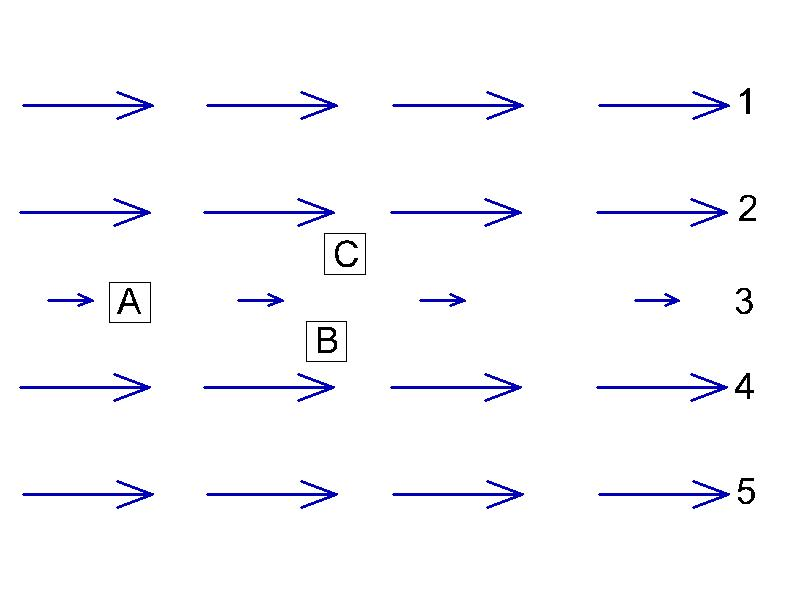
\includegraphics[width=1\linewidth]{./graphics/fig171}
\caption{Horizontal Vector Field}
\end{figure}

Along the horizontal direction, the vectors are the same in magnitude and direction. Going down vertically across, the magnitude changes for 2 to 3 and 3 to 4. 1 to 2 and 4 to 5 remains same. A small area \textbf{A} placed at the location shown, can create some kind of shear on the object depending on the strength of the vector through the top and bottom of \textbf{A}, less \textbf{A} be at \textbf{B}. \textbf{B} will turn counterclockwise while \textbf{C} will turn clockwise as the force created by the arrow magnitude is more at the top for \textbf{C} compared to the bottom of \textbf{C} and more at the bottom of \textbf{B} compared to the top. Hence rotation is experienced in that region. If we however consider a field shown below. That is the field magnitude is changing in the \textbf{x} direction.
\begin{figure}[h]
\centering
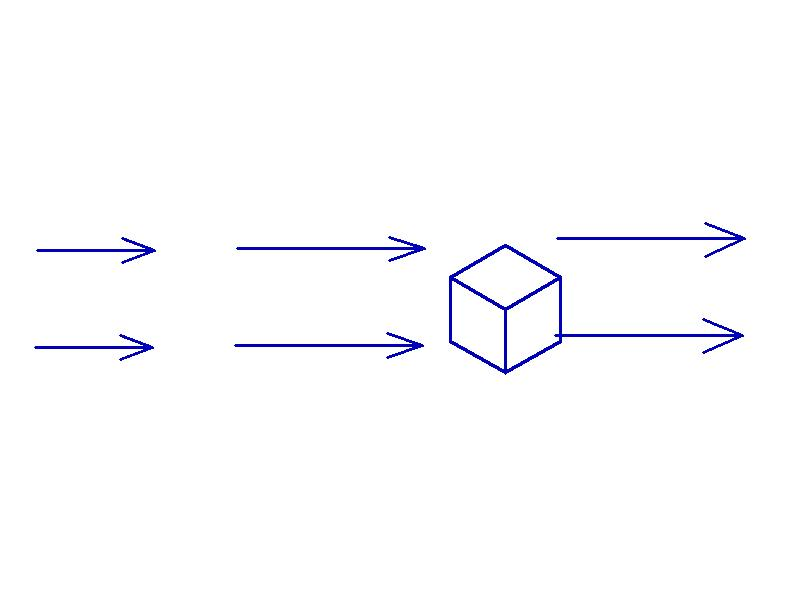
\includegraphics[width=1\linewidth]{./graphics/fig172}
\caption{Changing Field Magnitude}
\end{figure}

If we put a small volume in this region and treat the field like fluid flow velocity with increasing velocity of fluid as we move towards the right as shown by the magnitude of the arrow. The fluid going into the box has more value than what is coming out of the box. Hence there is a net outward flow of fluid from this volume. This kind of field will have a divergence.

Divergence is the best way to capture the effect of something either flowing out of a volume (oozing out) and the direction can be positive (net flow out of the volume) or negative (net flow into the volume).

Looking at this phenomenon where some rotation is involved, the phenomenon which can capture the effect is the \textit{curl}. Divergence and curl are the mathematical operations which capture these phenomenon.

We see later when we go into electromagnetic fields, that the concept of physics are mathematically captured by the curl and divergence operators.

\section{Laplacian operator}
Another operator defined in terms of the del operator $\nabla$ is called the \textbf{Laplacian Operator}. It is a second-order operator denoted as $\nabla^2 = \nabla \cdot \nabla$.

If we take the $\nabla$ as a vector operator, then the dot product of the two $\nabla$ operators is given by $\nabla^2$ and it becomes a scalar operator.

\begin{dmath}
\nabla \cdot \nabla =  \left(\frac{\partial  }{\partial x}\hat x + \frac{\partial  }{\partial y}\hat y + \frac{\partial  }{\partial z}\hat z \right) \cdot \left( \frac{\partial  }{\partial x}\hat x + \frac{\partial  }{\partial y}\hat y + \frac{\partial  }{\partial z}\hat z\right)
\end{dmath}

\begin{dmath}
\frac{\partial^{2}  }{\partial x^{2}}\hat x + \frac{\partial^{2}  }{\partial y^{2}}\hat y + \frac{\partial^{2}  }{\partial z^{2}}\hat z = \nabla^{2} = \nabla \cdot \nabla
\end{dmath}

So the laplacian operator is a second order differential operator and the operator is a scalar operator. So to operate on a scalar quantity, it becomes $\nabla\cdot\nabla$(scalar quantity).\newline

For a Scalar function $F$, $\nabla^2f = \nabla \cdot (\nabla f)$ but $\nabla f =$ gradient of scalar function of $f$. And the dot product in $\nabla \cdot (\nabla f) $ stands for divergence of the gradient of $f$.

$\nabla^2 f= \nabla .\cdot (\nabla f) =$ Divergence of gradient of the scalar function. The $\nabla^2 $ operator is not restricted to the scalar function only, it can operate also on vectors as $\nabla^2 \overline{F} = \nabla \cdot \nabla \overline{F}$ but this will not have meaning as we have not defined what $\nabla \overline{F}$ is.
\begin{figure}[h]
\centering
\begin{minipage}{.25\textwidth}
\centering
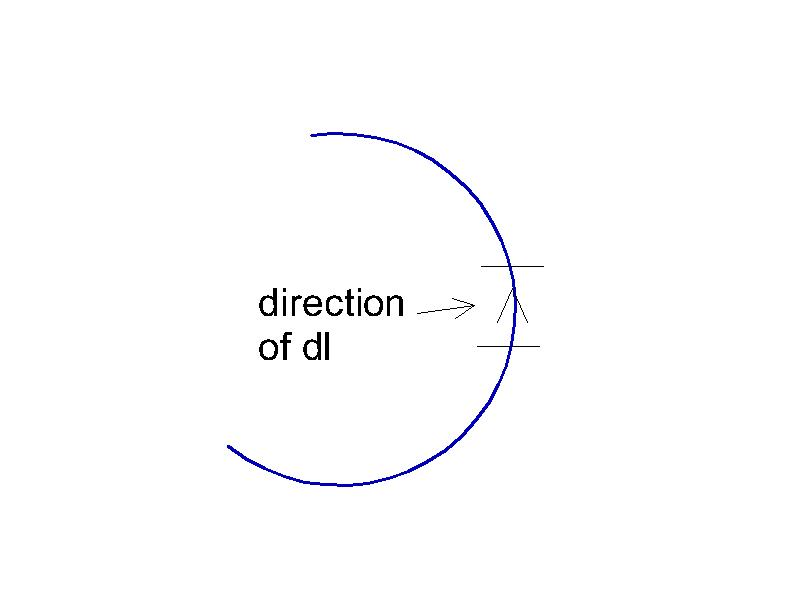
\includegraphics[width=.4\linewidth]{./graphics/fig173}
\label{fig:fig173}
\end{minipage}%
\begin{minipage}{.25\textwidth}
\centering
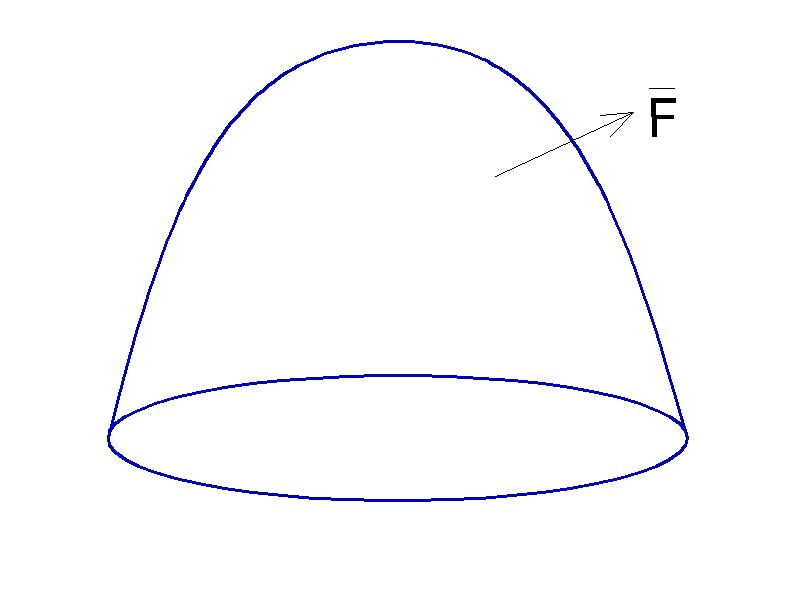
\includegraphics[width=.4\linewidth]{./graphics/fig173b}
\label{fig:fig173b}
\end{minipage}
\begin{minipage}{.5\textwidth}
\centering
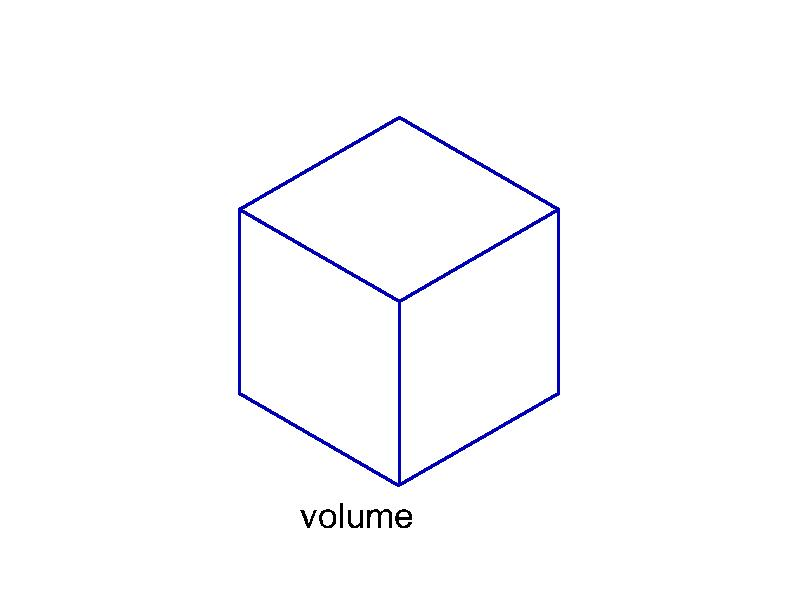
\includegraphics[width=.4\linewidth]{./graphics/fig173c}
\label{fig:fig173c}
\end{minipage}%
\caption{line surface and volume integration}
\end{figure}

The DEL operator $\nabla$ can operate as either divergence or a curl. So in this case, we take $\nabla^2$ and operate it directly on the vector quantity so that:
\begin{dmath}
\nabla^{2} \overline{F} = \frac{\partial ^ {2}}{\partial x^{2}}(\overline{F}) + \frac{\partial ^ {2}}{\partial y^{2}}(\overline{F}) + \frac{\partial ^ {2}}{\partial z^{2}}(\overline{F})
\end{dmath}
That is we take the second order differential of all the components that make up $\overline{F}$ i.e
\begin{equation*}
\overline{F} = F_{x}\hat x + F_{y}\hat y + F_{z}\hat z
\end{equation*}
So that
\begin{dmath}
\nabla^{2} \overline{F} = \frac{\partial ^ {2}}{\partial x^{2}}(F_{x}\hat x + F_{y}\hat y + F_{z}\hat z) + \frac{\partial ^ {2}}{\partial y^{2}}(F_{x}\hat x + F_{y}\hat y + F_{z}\hat z) + 
\frac{\partial ^ {2}}{\partial z^{2}}(F_{x}\hat x + F_{y}\hat y + F_{z}\hat z)
\end{dmath}
Then we combine individual components to have
\begin{dmath*}
\nabla^{2}F = (\frac{\partial ^{2} Fx}{\partial x^2} + \frac{\partial ^{2} Fx}{\partial y^2} + \frac{\partial ^{2} Fx}{\partial z^2})\hat{x} + (\frac{\partial ^{2} Fy}{\partial x^2} + \frac{\partial ^{2} Fy}{\partial y^2} + \frac{\partial ^{2} Fy}{\partial z^2})\hat{y} + (\frac{\partial ^{2} Fz}{\partial x^2} + \frac{\partial ^{2} Fz}{\partial y^2} + \frac{\partial ^{2} Fz}{\partial z^2})\hat{z}
\end{dmath*}
\begin{dmath}
\nabla^{2}F_x \hat x + \nabla^{2}F_y \hat y + \nabla^{2}F_z \hat z = \nabla^{2}\overline{F}
\end{dmath}
Later we shall see that this operation will be required when solving the problem of electro-magnetics.

\section{Integral Operators}

We have been dealing with differential operators up to this point now we have to deal with integral operators which has to do with Integration of the vector fields. If we have a vector field, there is a possibility that we can take the integral of this vector fields in a plane or along the contour or along a path.It is possible that we can take the integration of this vector on a surface which can be an open or closed surface. Or we can take the integral over a volume. 

% insert image here
When we do the integration along a path, it is called \textbf{Contour Integration}, while integration over a surface we call \textbf{Surface Integration}. And since a surface is two dimensional in nature, we have a double integral.

So a contour integration is a single integration, for a volume integration, it will be a triple integration i.e in the three dimensional space.

We have important theorems which connect line integrals to surface integrals and surface integrals to volume integrals. We may need to to change from one type of integral to another integral type e.g from line integral to surface integral or from surface integral to volume integral.

It should be kept in mind however that integral is a Scalar quantity. Thus the final answer after integration will always be a Scalar quantity. We can define line, surface and volume integration if we take some vector $\overline{A}$ i.e $\overline{A}$ is a vector field, then the line integration around some path C is ${\displaystyle \int  \overline{A} \cdot \overline{dl}}$. If we integrate along the contour in the direction shown, $dl$ has both magnitude and direction. If the path is a closed path, or mathematically we say if the contour is a closed contour, we have a closed line integral $= {\displaystyle \oint  \overline{A} \cdot \overline{dl}}$.
\begin{equation}
{\displaystyle \int  \overline{A} \cdot \overline{dl} = }open\; contour \newline  {\displaystyle \oint  \overline{A} \cdot \overline{dl}= }closed\; contour
\end{equation}
So at every location $\overline{A}$ we find out the product $\overline{A} \cdot \overline{dl}$ and sum it all up. This is the basis for the line integral.
\section{Surface Integral for Infinitesimally small Area}
We can carry out similar operation for the surface integral as having an area $A$ with an infinitesimally small area $d\overline{A}$. $d\overline{A}$ has direction perpendicular to that small area, if the vector field in this area is $\overline{A}$, we can define the surface integration as:
%insert integration image here
(the surface may be closed or open, here it is an open surface).

Surface Integral =
\begin{equation*}
{   \iint \overline{A} \cdot d\overline{A}= open surface }
\end{equation*}
\begin{equation}
\oiint \overline{A} \cdot d\overline{A} = closed surface
\end{equation}

d$\overline{A}$ is a scalar quantity so that the integration is also a scalar quantity. Now the direction for $d\overline{A}$ is thus. If it is a closed surface, the direction of the normal is taken as the outward normal for the volume created by the closed surface and it is in the positive normal direction.

If it is an Open Surface there is no preference for defining the $unit$ $normal$. We can define the $unit$ $normal$ in either direction.

\begin{figure}
\centering
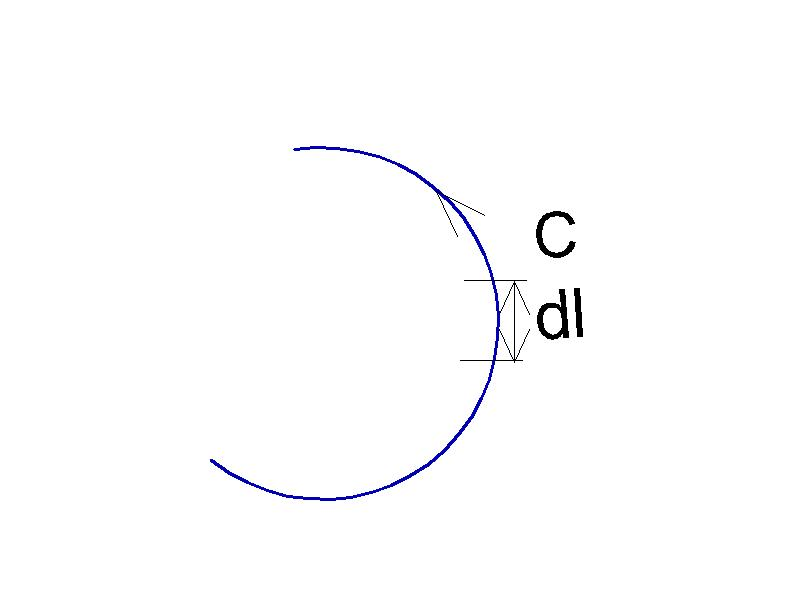
\includegraphics[width=0.7\linewidth]{./graphics/fig174}
\caption{Open and closed contour}
\label{fig:open-and-closed-contour}
\end{figure}

$n_1$ and $n_2$ are valid unit normal for Surface \textbf{S}.

However, later on when we try to connect the contours to the surface for open surface, then at that time we follow the convention of right hand rule. That is for any open surface to know the positive unit normal, just let the curl of the finger go counter-clockwise around the surface, the direction to the thumb points in the positive direction of unit normal to that surface.
%insert image

The third is the volume integral,if we have some function which is a Scalar $f$:
\begin{dmath*}
\text{Volume integral} = \iiint fdV
\end{dmath*}

Now when we try to relate the different integrations, the line integral to surface integral and surface integral to volume integral, essentially the vector fields are operated on by the DEL $\nabla$ operators, then there is a relationship between these del operated fields in the integration domain. So two important theorems essentially relate this i.e they are called the \textbf{Divergence theorem} and the \textbf{Stokes theorem}.

\section{Divergence Theorem}

This converts a surface integral for a vector field to a volume integral. If we have a vector field $\overline{A}$, then the divergence theorem states that for a \textbf{closed surface}, we have that:
\begin{equation}
\oiint \overline{A} \cdot \overline{da} = \iiint (\nabla \cdot \overline{A})dV
\end{equation}
%insert images here

So if we have a volume bounded by surface $S$, if we have a vector $\overline{A}$ and we know the surface integral of this vector i.e $\oiint \overline{A}\cdot\overline{da}$, it can be converted into a volume integral.
\begin{figure}
\centering
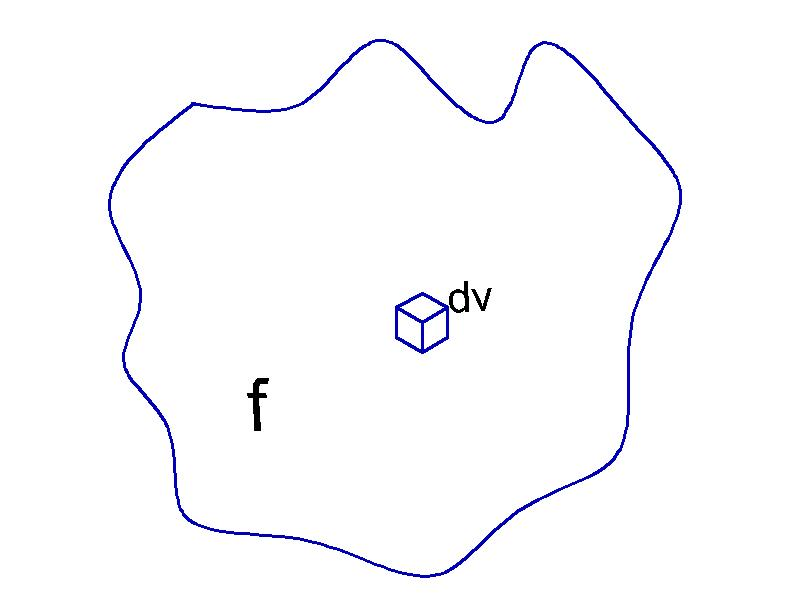
\includegraphics[width=0.7\linewidth]{./graphics/fig175}
\caption{closed line to open surface }
\label{fig:page-8}
\end{figure}


So $\oiint \overline{A} \cdot \overline{da} = \iiint (\nabla \cdot \overline{A})dV$ is called the divergence theorem. So when we have to convert between closed surface integral and volume integral, these theorems come very handy.

\section{Stokes Theorem}
It converts a closed line integral to an open surface integral or vice-versa. 
\begin{figure}[h]
\centering
\begin{minipage}{.25\textwidth}
\centering
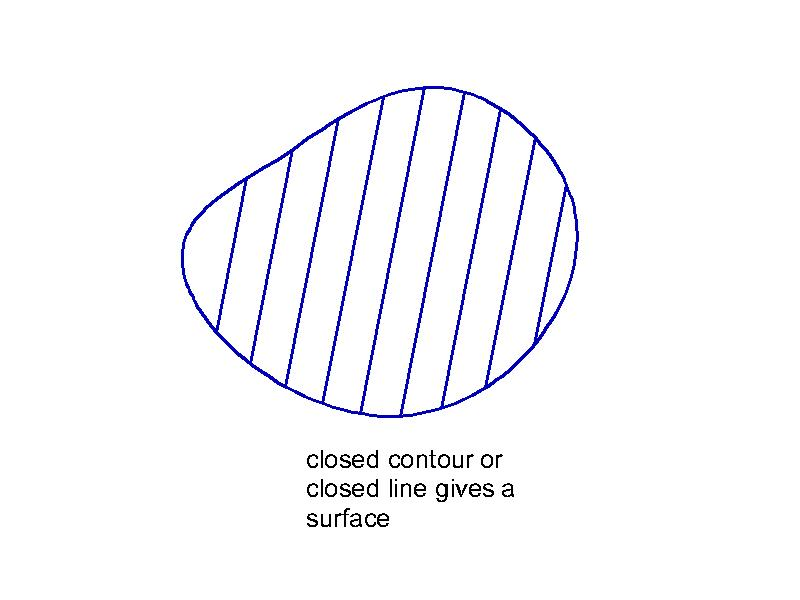
\includegraphics[width=.4\linewidth]{./graphics/fig176}
\label{fig:fig176}
\end{minipage}%
\begin{minipage}{.25\textwidth}
\centering
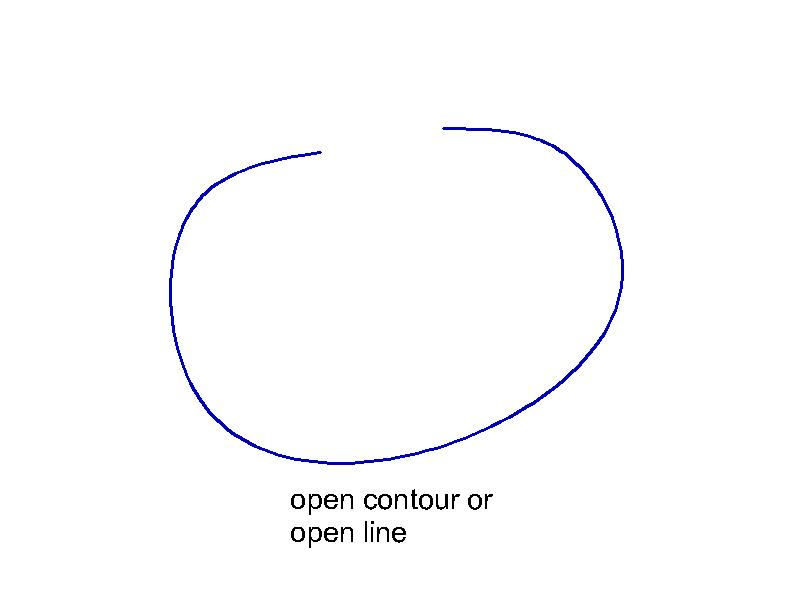
\includegraphics[width=.4\linewidth]{./graphics/fig176b}
\label{fig:fig176b}
\end{minipage}
\begin{minipage}{.5\textwidth}
\centering
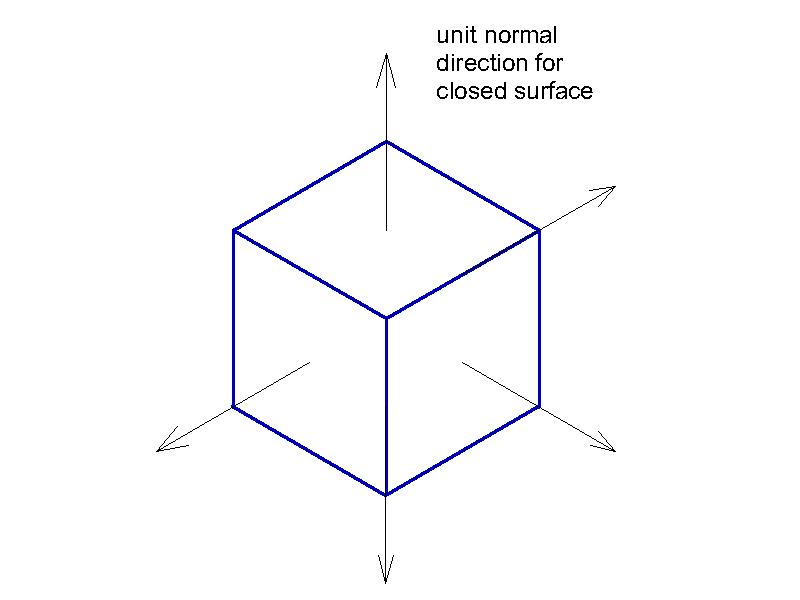
\includegraphics[width=.4\linewidth]{./graphics/fig176c}
\label{fig:fig176c}
\end{minipage}%
\caption{surface integral to volume integral conversion}
\end{figure}

The surface shown is open and we have the boundary defined by contour $C$. Now we can have a small area with unit vector $\hat n$.

Then we can have the contour $C$ for which line integral was defined for vector $\overline{A}$, so how do we define the path $C$ wrt $\hat n$. The convention is we follow the right hand rule, if our contour as shown is going clockwise $\hat n$ goes outward, if it goes anticlockwise $\hat n$ goes inward.

Let us illustrate this better with a very clear diagram. 
\begin{figure}[h]
\centering
\begin{minipage}{.25\textwidth}
\centering
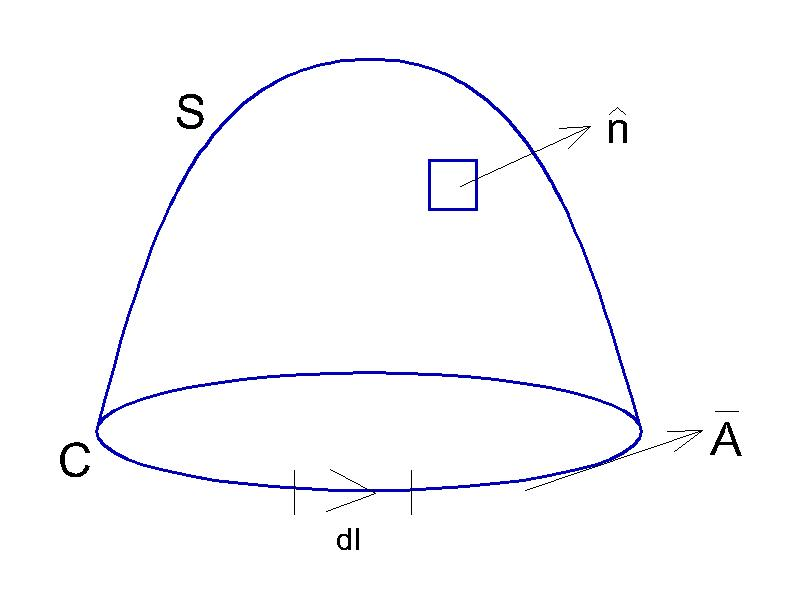
\includegraphics[width=.4\linewidth]{./graphics/fig177}
\label{}
\end{minipage}%
\begin{minipage}{.25\textwidth}
\centering
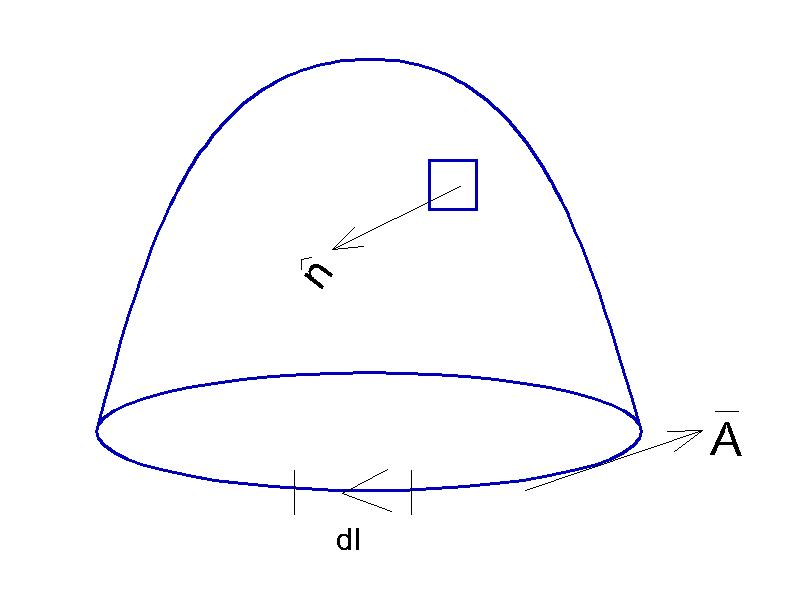
\includegraphics[width=.4\linewidth]{./graphics/fig177b}
\label{}
\end{minipage}
\begin{minipage}{.5\textwidth}
\centering
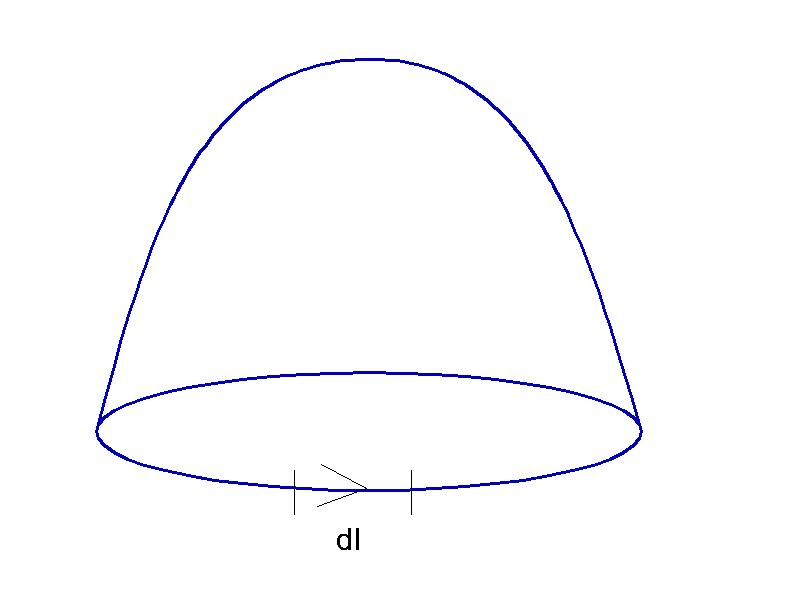
\includegraphics[width=.4\linewidth]{./graphics/fig177c}
\label{}
\end{minipage}%
\caption{contour integration}
\end{figure}

Note that the bottom of the surface is open as compared to when this was not the case in the divergence theorem example. For these open surface $S$ bounded by closed contour $C$ the Stokes theorem states that:
\begin{equation}
\oint_c \overline{A} \cdot \overline{dl} = \iint_s  (\nabla \times \overline{A})\cdot\overline{da}
\end{equation}

So this theorem can be used to convert a line integral to surface integral or vice-versa.

\section{Summary}
To summarize all these again, if we have a closed surface, the closed surface integral and the volume integral in that closed surface can be related by the divergence theorem.
\begin{equation}
\oiint \overline{A}\cdot\overline{dA} = \iiint_v(\nabla\cdot\overline{A})dV
\end{equation}
For an open surface whose boundary at the open end is defined by a closed line path or contour, the line integral of that closed contour and the surface integral in the open surface are related by $Stokes$ $Theorem$.
\begin{equation}
\oint\overline{A}\cdot\overline{dl} = \iint_s(\nabla\times\overline{A})\cdot\overline{da}
\end{equation}	
Later on for solving the problem of electro-magnetics, when we write $Maxwell's Equation$ in integral and differential forms, the two theorems become very important and becomes handy in converting from integral to differential forms. Having understood the basics of vectors, now we can go to the basic quantities of electro-magnetics which we are going to make use of in further analysis, that is the quantity like electric and magnetic fields.\newline
The origin of the electromagnetic phenomenon is based on the basic $CHARGE$. So if we consider a charge, we know in form of $coulombs$ law that the charge has an effect all around it. If you put a charge in the vicinity of that charge, it experiences a force. This quantity is measured by an effect called called the $Electric$ $Field$.
So if we take a charge and go in the vicinity of that charge, we experience a force which is characterized by a quantity called \textbf{electric field}. However if we put this charge in motion, then it constitute a current as current is nothing but the movement of charge or rate of change of charge.\newline
So if the charge starts moving, that means you have a sustained flow of charges that gives you current and then you have magnetic fields. So some charge when it is steady or stationary it gives you electric field, when it starts moving, it gives you current and that gives you magnetic field.\newline
The charge can accelerate also, then if we accelerate the charges, then it gives you electric and magnetic field. So essentially we are dealing with these quantities here; the charges, current, electric and magnetic fields and try to establish the relationship between these quantities. The relationship we have between these quantities is given by what is called MAXWELL'S EQUATIONS. So essentially now starting with the basics of these quantities, we would try to establish a relationship between these laws of physics in mathematical form using vector notation and vector theorems which we establish, we get the maxwell's equation. So the quantity which we have now as the first quantity is Electric Field $\overline{E}$ which is nothing but the force per unit charge, the electric field is a vector quantity. It has both magnitude and direction. It has V/m as its unit. Then we have a media property. Lets say we measure electric field in a vacuum, we experience a certain force on a unit charge. If we measure the same thing and change the medium parameter to some other dielectric, then the force measured will change. So the quantity which does not depend on any parameter is the electric displacement vector $\overline{D}$.
So electric field is a quantity which is related to the charge producing the field and is also affected by the medium parameter which is called permittivity of the medium. So we have a medium parameter called permittivity $\varepsilon$ and has unit Farad/m. If the medium parameter changes, the permittivity changes and the electric field $\overline{E}$ measured at that point changes. Permitivity of vacuum or free space is denoted by $\varepsilon_{0} =\frac{1}{36\pi}$ $\times 10^{-9}F$. Sometimes written as 8.86$\times10^{-12}F/m.$
If we take another medium whose permittivity is $\varepsilon$, the ratio $\frac{\varepsilon}{\varepsilon_{0}}$ is what is called the dielectric constant for the material or relative permittivity. 
Dielectric constant $\varepsilon_{r}\equiv$ relative permittivity= $\frac{\varepsilon}{\varepsilon_{0}}$.
The quantity which is independent of medium parameter is the displacement vector $\overline{D}=\varepsilon \overline{E}$

For a given property change, the $\overline{E}$ changes, $\overline{D}$ remains the same, as it only depends upon the charge which is creating the field. The quantity $\varepsilon$ in a general medium can be constant everywhere or it can vary as a function of space in three dimensional space. It can also depend on the direction, that means if we measure permittivity in x direction, its value may vary from that in the y and z direction. So in general, the quantity  $\varepsilon$  can be direction dependent, or it may be space dependent. When  $\varepsilon$  varies as a function of space, we call the medium \textbf{INHOMOGENOUS MEDIUM}. If  $\varepsilon$  is direction dependent, then the medium is called an ANISOTROPHIC MEDIUM. If  $\varepsilon$ does not vary as a function of space, we call it \textbf{HOMOGENOUS MEDIUM}. If it does not vary with direction, we call that medium \textbf{ISOTROPHIC MEDIUM}
However we will be dealing with a media that is homogenous and isotropic. This means that the dielectric constant of the medium, which we shall consider, has  $\varepsilon$ that is constant in space and does not change with direction. However, if  $\varepsilon$  was anisotrophic, then  $\varepsilon$  becomes a $3\times 3$ matrix of  $\varepsilon$  multiplied by vector $\overline{E}$ . For isotrophic medium  $\varepsilon$  is a scalar quantity. So for this course, we deal with medium where  $\varepsilon$  is a scalar quantity.
So in a homogenous and isotrophic medium,  $\overline{D}$ is a scalar version of  $\overline{E}$. Comparing  $\overline{D}$ and  $\overline{E}$, they have different magnitude but with the same direction. However, if the medium were to be anisotrophic,  $\varepsilon$ is a $3\times 3$ matrix and it rotates the vector  $\overline{E}$ and in general  $\overline{D}$ and  $\overline{E}$ are not in the same direction.
\begin{figure}[h]
\centering
\begin{minipage}{.25\textwidth}
\centering
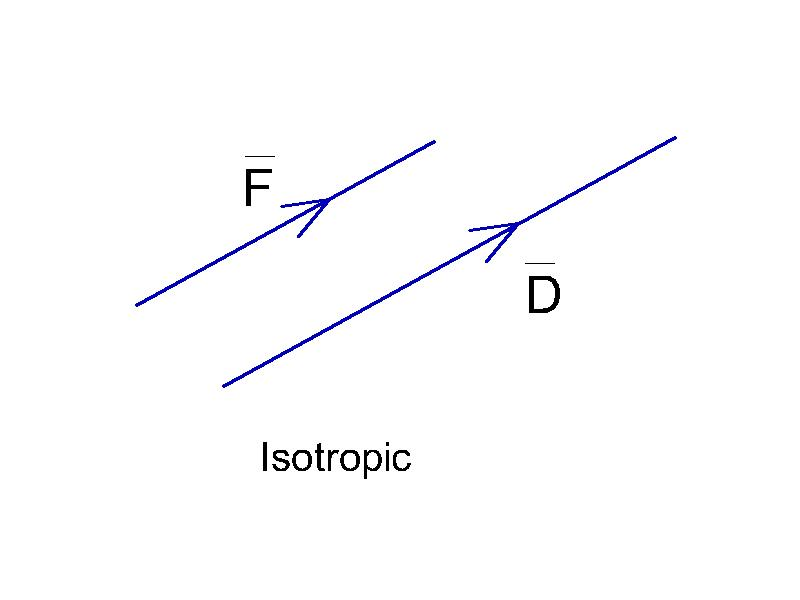
\includegraphics[width=.4\linewidth]{./graphics/fig178b}
\label{fig:fig178b}
\end{minipage}
\begin{minipage}{.25\textwidth}
\centering
 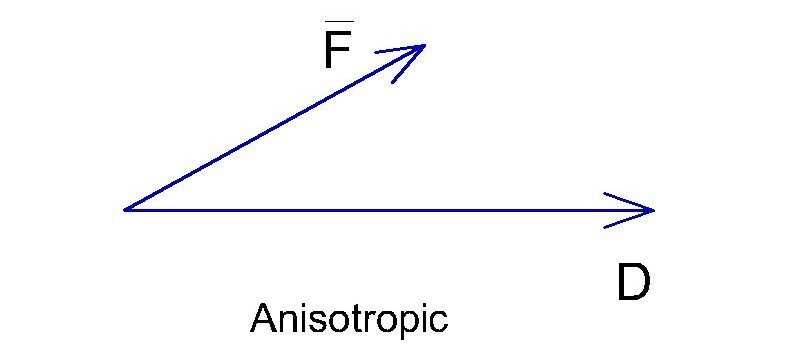
\includegraphics[width=.4\linewidth]{./graphics/fig178}
\label{fig:fig178a}
\end{minipage}
\caption{Isotrophic and Anisotrophic Medium}
\end{figure}

Now we have another quantity which is very useful that we have to define ; the \textbf{Electric Potential} of the field. The electric field is related to the electric  potential V (scalar ) by 
$\overline{E}$= -$\nabla $ V.
So if we know potential at a point, we can take the gradient to get the Electric field at that location. From here we get the unit of electric field. So if we find the potential, the unit of V is Volts. The del operator is a differential spatial operator$\frac{d}{dx}$ ; i.e $\frac{1}{l} or\frac{1}{m}$ that gives unit of electric field, which is V/m. So this relation of finding out electric field from the potential comes very handy whenever we want to find electric field in a general complex distribution of charges. If we find the electric field  $\overline{E}$ at a particular location and find the component of the electric field for each of the charges which are distributed in space, we carry out vector additions at that point for the electric fields. It is however easier to find the potential of the different charges and add them together. The negative gradient of that gives you the electric field. So these are the basic quantities for representing the electrostatic parameters ; the electric field  $\overline{E}$ and the electric potential V.
